\documentclass[border=1pt,tikz,varwidth=\maxdimen]{standalone}

\usetikzlibrary{positioning,calc,matrix}

\usepackage{amsmath,mathtools}

\begin{document}
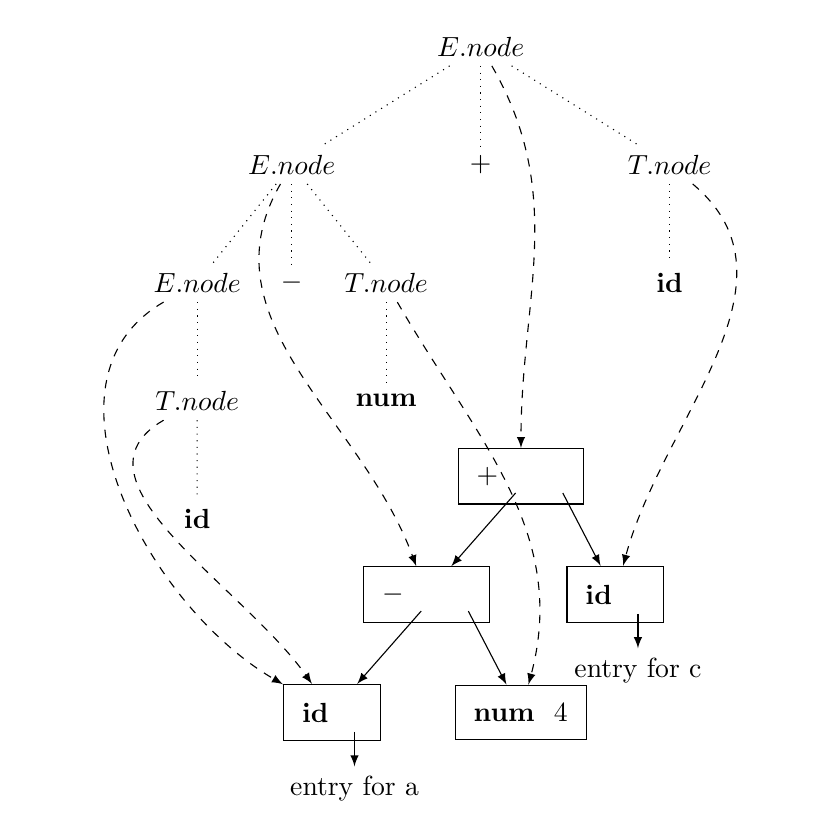
\begin{tikzpicture}[
  tree_node/.style={draw,matrix,matrix of nodes,ampersand replacement=\&,nodes={minimum width=1.21em}},
  level/.style={sibling distance=2.4cm/#1},
  emph1/.style={edge from parent/.style={dotted,draw}},
  emph2/.style={edge from parent/.style={dashed,draw}},
  norm/.style={edge from parent/.style={solid,draw}}
  ]
  \node (NRoot) {\(E.node\)}
  child[emph1] {
    node (N1L) {\(E.node\)}
    child {
      node (N1L2L) {\(E.node\)}
      child {
        node (N1L2L3) {\(T.node\)}
        child {
          node (N1L2L34) {\bf id}
        }
      }
    }
    child {
      node (N1L2M) {\(-\)}
    }
    child {
      node (N1L2R) {\(T.node\)}
      child {
        node (N1L2R3) {\bf num}
      }
    }
  }
  child[emph1] {
    node (N1M) {\(+\)}
  }
  child[emph1] {
    node (N1R) {\(T.node\)}
    child {
      node (N1R2) {\bf id}
    }
  };

  \node[below right=1.6em of N1L2R3,tree_node] (add) {\(+\) \& {} \& {}\\}
  child {
    node[tree_node] (sub) {\(-\) \& {} \& {} \\}
    child {
      node[tree_node] (ida) {{\bf id} \& {} \\};
    }
    child[missing]
    child {
      node[tree_node] (num) {{\bf num} \& {4} \\};
    };
  }
  child[norm] {
    node[tree_node] (idc) {{\bf id} \& {} \\};
  };
  \draw[-latex] (add-1-2) -- (sub);
  \draw[-latex] (add-1-3) -- (idc);
  \draw[-latex] (sub-1-2) -- (ida);
  \draw[-latex] (sub-1-3) -- (num);

  \draw[dashed,-latex] (NRoot)  to[out=300,in=90]  (add);
  \draw[dashed,-latex] (N1L)    to[out=240,in=110] (sub);
  \draw[dashed,-latex] (N1L2L)  to[out=210,in=150] (ida);
  \draw[dashed,-latex] (N1L2L3) to[out=210,in=125] (ida);
  \draw[dashed,-latex] (N1L2R)  to[out=300,in=75]  (num);
  \draw[dashed,-latex] (N1R)    to[out=320,in=75]  (idc);

  \draw[-latex] (idc-1-2) -- ++(0,-1.6em) node[anchor=north]{entry for c};
  \draw[-latex] (ida-1-2) -- ++(0,-1.6em) node[anchor=north]{entry for a};
\end{tikzpicture}
\end{document}
